\documentclass[12pt]{article}
\usepackage{amsmath}
\usepackage{amssymb}
\usepackage{graphicx}
\usepackage{hyperref}
\usepackage[latin1]{inputenc}
\usepackage{listings}
\usepackage{pgfplots}
\usepackage{hyperref}
\usepackage{geometry}
\renewcommand{\labelitemi}{$\textendash$}
\renewcommand{\arraystretch}{1.4}
\hypersetup{colorlinks=true, urlcolor=cyan}
\geometry{
    a4paper,
    total={170mm,257mm},
    left=20mm,
    right=20mm,
    top=15mm,
    bottom=15mm
}

\title{\vspace{-5ex}ST3009: Mid-Term Assignment\vspace{-2.5ex}}
\author{Conor McCauley - 17323203}
\date{\vspace{-2ex}March 31, 2020\vspace{-2ex}}

\begin{document}

\maketitle

\section*{Question 1}

\noindent (a) The \texttt{pmf\_hist()} method from the code produces the following histogram for user 0:

\begin{center}
    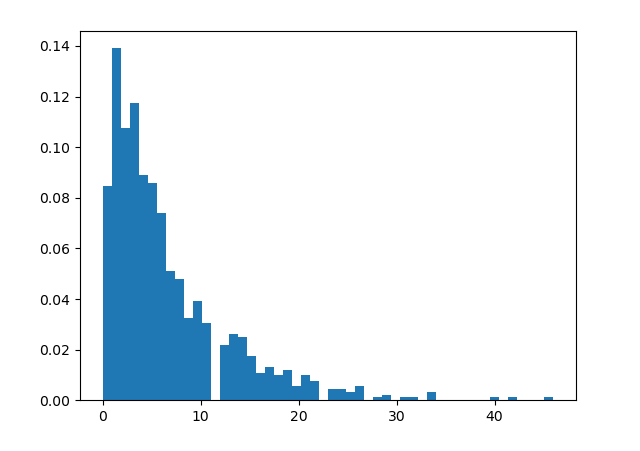
\includegraphics[scale=0.6]{q1_hist.png}
\end{center}

\noindent (b) The \texttt{prob()} method from the code calculates the total sum of $X_i$ and divides it by the number of timings to find the mean. It returns the following estimate for user 0:

$$ Prob(X_0 = 1) = 0.201 $$

\noindent (c) The \texttt{conf\_intervals()} and \texttt{conf\_intervals\_bootstrap()} methods estimate the 95\% confidence intervals using CLT/Chebyshev's inequality and bootstrapping, respectively. The bootstrapped methods run on 1000 random samples (with replacement) of 20\% of the dataset. They return the following estimates for user 0:

\begin{center}
    \begin{tabular}{|c|c|}
        \hline
        Chebyshev & $0.1443 \le X \le 0.2577$ \\ \hline
        CLT & $0.1757 \le X \le 0.2263$ \\ \hline
        Bootstrap Chebyshev & $0.1445 \le X \le 0.2579$ \\ \hline
        Bootstrap CLT & $0.1758 \le X \le 0.2265$ \\ \hline
    \end{tabular}
\end{center}

\indent Chebyshev's inequality gives us a looser bound than the CLT but it is an actual bound that works for any value of $N$. The CLT gives us a tighter bound but it is only an approximation related to the finite value of $N$. Bootstrapping, like the CLT, only provides an approximation. However, bootstrapping works even if the data is not normally distributed.

\section*{Question 2}

\noindent The method from question 1(b) returns the following estimates for each of the users:

\begin{center}
    \begin{tabular}{|c|c|c|}
        \hline
        $Prob(X_0 = 1) = 0.201$ & $Prob(X_3 = 1) = 0.436$ & $Prob(X_6 = 1) = 0.407$ \\ \hline
        $Prob(X_1 = 1) = 0.405$ & $Prob(X_4 = 1) = 0.215$ & $Prob(X_7 = 1) = 0.433$ \\ \hline
        $Prob(X_2 = 1) = 0.347$ & $Prob(X_5 = 1) = 0.221$ & $Prob(X_8 = 1) = 0.519$ \\ \hline
    \end{tabular}
\end{center}

\section*{Question 3}

\noindent The probability that some request $n$ takes longer than 10ms to complete, $P(Z_n > 10)$, is as follows:

$$P(Z_n > 10) = \sum_i P(Z_n > 10 \mid U_n = i) \cdot P(U_n = i)$$

\indent However, given that $P(Z_n > 10 \mid U_n = i)$ is just $Prob(X_i = 1)$ we can rewrite the sum like so:

$$P(Z_n > 10) = \sum_i Prob(X_i = 1) \cdot P(U_n = i)$$

\indent The \texttt{prob\_z()} method from the code return the following estimate: $P(Z_n > 10) = 0.338$.

\section*{Question 4}

\noindent Using Bayes' Rule we can calculate $P(U_n = 0 \mid Z_n > 10)$ as follows:

$$P(U_n = 0 \mid Z_n > 10) = \frac{P(Z_n > 10 \mid U_n = 0) \cdot P(U_n = 0)}{P(Z_n > 10)}$$
$$= \frac{Prob(X_0 = 1) \cdot P(U_n = 0)}{P(Z_n > 10)}$$
$$= \frac{0.201 \cdot 0.11281345252473}{0.33799}$$
$$= 0.06709$$

\section*{Question 5}

\noindent The \texttt{sim\_z()} method from the code runs 100,000 request simulations and, for each simulation:

\indent (1) randomly chooses which user the request came from using the given probabilities, and

\indent (2) randomly checks if the request took longer than 10ms using the chosen user's probability from question 2.

\noindent It returned $P(Z_n > 10) = 0.33806$, which is extremely close to the answer from question 3.

\indent The simulated value is approximately equal to the calculated value ($\pm0.017\%$) which tells me that the calculated results are correct. However, I noticed that when I ran the simulation with 10,000 requests the resulting value was, on average, around 35 times less accurate ($\pm0.355\%$) than the 100,000 request simulation.

\indent These differing results highlight an important question in stochastic simulations which is the trade-off between computing power and simulation accuracy: in this case it seems 100,000 random simulations is ideal as the results are very accurate and the simulation doesn't take more than a second to run (on my PC anyway).

\section*{Appendix I: Dataset}

\noindent The complete dataset that was used can be found \href{https://raw.githubusercontent.com/conormccauley1999/College/master/ST3009\%20-\%20Statistical\%20Methods\%20for\%20Computer\%20Science/Mid-Term\%20Assignment/dataset_raw.txt}{here} while the formatted datasets can be found \href{https://github.com/conormccauley1999/College/tree/master/ST3009\%20-\%20Statistical\%20Methods\%20for\%20Computer\%20Science/Mid-Term\%20Assignment}{here}. 

\section*{Appendix II: Code}

\noindent The code can also be found  \href{https://raw.githubusercontent.com/conormccauley1999/College/master/ST3009\%20-\%20Statistical\%20Methods\%20for\%20Computer\%20Science/Mid-Term\%20Assignment/code.py}{here}.

\begin{lstlisting}[language=Python]
from math import sqrt
from random import choices, uniform
import matplotlib.pyplot as plt

def parse_timings():
	return tuple(zip(*[list(map(int, line.strip().split())) \
		for line in open("dataset_timings.txt").readlines()]))

def parse_probabilities():
	return tuple(map(float, open("dataset_probabilities.txt")\
		.readline().split()))

def pmf_hist(timings):
	plt.hist(timings, 50, density=True)
	plt.show()

def prob(timings):

	rv = lambda x: 1 if x > 10 else 0
	count = sum(rv(timing) for timing in timings)

	return count / len(timings)

def conf_intervals(timings):

	N = len(timings)
	mu = prob(timings)
	sigma = sqrt(mu - (mu ** 2))

	cheb_lo, cheb_hi = mu - (sigma / sqrt(0.05 * N)), \
	mu + (sigma / sqrt(0.05 * N))
	clt_lo, clt_hi = mu - (2 * (sigma / sqrt(N))), \
	mu + (2 * (sigma / sqrt(N)))

	print("95%% CI - Chebyshev: %.4f <= X <= %.4f" % \
		(cheb_lo, cheb_hi))
	print("95%% CI - CLT: %.4f <= X <= %.4f" % \
		(clt_lo, clt_hi))

def conf_intervals_bootstrap(timings):
	
	N = len(timings)
	S = 1000
	
	# sample 20% of dataset (with replacement) 1000 times
	means = []
	for i in range(S):
		sample = choices(timings, k=int(0.2 * N))
		means.append(prob(sample))

	mu = sum(means) / len(means)
	sigma = sqrt(mu - (mu ** 2))
	
	cheb_lo, cheb_hi = mu - (sigma / sqrt(0.05 * N)), \
	mu + (sigma / sqrt(0.05 * N))
	clt_lo, clt_hi = mu - (2 * (sigma / sqrt(N))), \
	mu + (2 * (sigma / sqrt(N)))

	print("95%% CI - BS Chebyshev: %.4f <= X <= %.4f" % \
		(cheb_lo, cheb_hi))
	print("95%% CI - BS CLT: %.4f <= X <= %.4f" % \
		(clt_lo, clt_hi))

def prob_z(all_timings, probs):
	return sum(prob(all_timings[i]) * probs[i] \
		for i in range(len(all_timings)))

def sim_z(all_timings, prob_request):

	prob_timing = list(map(prob, all_timings))

	S = 100000
	count = 0
	for _ in range(S):

		# what user did the request come from?
		user_prob = uniform(0, 1)
		user_i = -1
		prob_sum = 0
		for i in range(len(prob_request)):
			prob_sum += prob_request[i]
			if user_prob <= prob_sum:
				user_i = i
				break

		# did the request take longer than 10ms?
		req_prob = uniform(0, 1)
		if req_prob <= prob_timing[user_i]:
			count += 1

	return count / S

# Data
all_timings = parse_timings()
probs = parse_probabilities()

# Q1(a)
pmf_hist(all_timings[0])

# Q1(b)
print(prob(all_timings[0]))

# Q1(c)
conf_intervals(all_timings[0])
conf_intervals_bootstrap(all_timings[0])

# Q2
for timings in all_timings[1:]:
	print(prob(timings))

# Q3
print(prob_z(all_timings, probs))

# Q5
print(sim_z(all_timings, probs))
\end{lstlisting}

\end{document}
